\documentclass[12pt]{article}
\usepackage{amsfonts, epsfig}
\usepackage[authoryear]{natbib}
\usepackage{graphicx}
\usepackage{fancyhdr}
\pagestyle{fancy}
\lfoot{\texttt{comsm0021.github.io}}
\lhead{Neural Information Processing - 7\_Daw\_EtAl - Conor}
\rhead{\thepage}
\cfoot{}
\begin{document}

\section*{A Kalman filter model of decision making}

One interesting aspect of decision making in humans and other animals,
is that it appears to place a value on information. This is often
described using the example of someone living in a village with two
night clubs. Imagine this person goes out one Thursday and chooses one
of the two night clubs, The Oasis, say and has a terrible night, awful
music, fighting on the dance floor and so on. The next Thursday night
they go to the other night club, The Warwick say, and have a great
time, everyone dancing at the disco, having a great time, nice curry
in the meal room\footnote{In the old days night clubs were required by
  licensing laws to serve a meal though few people ever ate them}. In
an unchanging world, the best thing to do from then on would be to go
to The Warwick every Thursday, it is the better night club after all.

However, the world is not unchanging\footnote{In fact the real Warwick
  this story is based on has now been demolished, an old folks home
  has been built where it once stood} if they did keep going to The
Warwick they might loose out, The Warwick might go down hill, employ a
bad DJ and aggressive bouncers and stop replacing the little mirrors
in their disco ball when these same little mirrors fall out. At the
same time, The Oasis might get its act together, might stop playing
Europop and might discourage dance-floor fighting\footnote{The real
  Oasis this story is based on never got its act together and remained
  a bad night spot until it closed}. The village person at this point
would be going to the wrong night club. Obviously the correct thing to
do is to sometimes make a decision that is not based on the optimal
predicted reward because the reward is to gain information about the
current state of the world.

There is now a very general theory of decision making call the Free
Energy Principle that attempts to model the value of knowledge. Here,
we will look at a more restricted attempt, in \citet{DawEtAl2006}, to
model what is called \textsl{exploration versus exploitation}, the
trade-off between exploiting a known resource and exploring in search
of a new one. In this paper they examine a number of different
models\footnote{Note that most of the actual details for this paper
  appear in the supplementary materials section}, but the one that
seems to work best is based on a so-called \textsl{soft-max} rule.

If there are $n$ alternative actions, with predicted average reward $\tilde{mu}_i$ for
the $i$th action, then a soft-max rule says that the $i$th action is
selected with probability
\begin{equation}
p_i=\frac{e^{\beta \tilde{\mu}_i}}{\sum_j e^{\beta \tilde{\mu}_j}}
\end{equation}
$\tilde{\mu}_i$ is used since $\mu_i$ without the $\sim$ is reserved
for the actual, rather than predicted reward.  Here $\beta$ is a
parameter which determines the amount of exploration, for large
$\beta$ then the action with the largest reward will have a $p_i$ near
to one, whereas for $\beta=0$ all the probabilities are equal; this
$\beta$ should respond to the predictibility of the environment with
$\beta$ increasing if the world is more predictable. $\beta$ might be
controlled by neuromodulation. However, that is another question, the
one of interest here is to fit this model and to compare it to other
models, such as one where the probabilities are
\begin{equation}
p_i=\left\{\begin{array}{ll}1-\epsilon&\tilde{\mu}_i\mbox{ is the
  biggest }\tilde{\mu}_j\mbox{
  value}\\\epsilon/n&\mbox{otherwise}\end{array}\right.
\end{equation}
The difficulty is to work out what the predicted rewards,
$\tilde{\mu}_i$, are.

\subsection*{An $n$-armed bandit}

\begin{figure}[htb]
\begin{center}

\includegraphics[width=4cm]{fig_one_armed.jpg}
\end{center}
\caption{A one-armed bandit. [Image from ebay]\label{fig_one_armed}}
\end{figure}

\citet{DawEtAl2006} describes a so-called $n$-\textsl{armed bandit}
task, named after the \lq{}one-armed bandit\rq{} gambling machine as
in Fig.~\ref{fig_one_armed}. In the experiment a subject has a choice
of four buttons to press. Each button has a reward, but the amount is
different for each button and the amount for each button varies with
time. In fact the mean reward is changed from trial to trial according to a
discrete Ornstein-Uhlenbeck process, that is a kind of mean-reverting
Gau\ss{}ian random walk:
\begin{equation}
\mu_i(t+1)=\lambda \mu_i(t)+(1-\lambda)\mu_0+v
\end{equation}
where $t$ is the trial number, $\mu_0$ is the initial value for the mean,
$\lambda$ is a parameter controlling how rapidly the mean reward heads
towards $\mu_0$ and $v$ is drawn independently for each trial from a
zero mean Gau\ss{}ian with variance $\sigma_v^2$. The actual reward
for a trial $t$ is then chosen to be
\begin{equation}
r_i(t)=\mu_i(t)+w
\end{equation}
where $w$ is also a zero mean Gau\ss{}ian with variance $\sigma_w^2$.
A schematic for the experiment is showing in Fig.~\ref{fig_daw_exp}.

\begin{figure}[htb]
\begin{center}
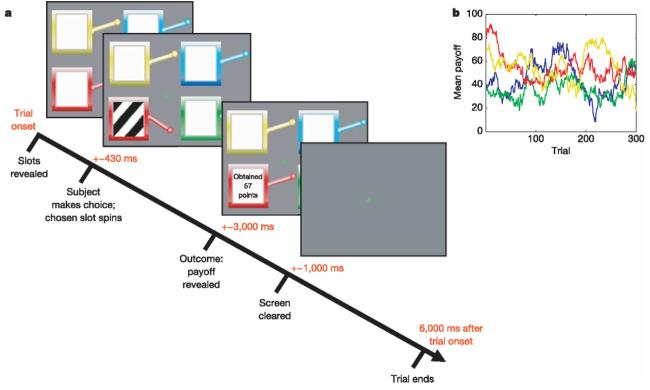
\includegraphics[width=12cm]{fig_daw_exp.jpg}
\end{center}
\caption{A schematic for the $n$-armed bandit task, \textbf{b} shows examples of how the mean rewards $\mu_i(t)$  evolve. [Image from \citep{DawEtAl2006}]\label{fig_one_armed}}
\end{figure}

Now the idea presented in the paper is that the subject estimates
$\mu_i$ using a one-dimensional Kalman filter: $\tilde{\mu}_i(t)$ is
the predicted mean reward for button $i$ at trial $t$. According to
their model the subject has an estimates of $\lambda$ and $\mu_0$
which we will call $\tilde{\lambda}$ and $\tilde{\mu}_0$; this is
slightly different from the derivation of the Kalman filter we looked
at before where we updated the speed from step to step. Thus from one
trial to the next the estimate $\tilde{\mu}_i$ is updated according to
\begin{equation}
\tilde{\mu}_i^-(t+1)=\tilde{\lambda}\mu_i(t)+(1-\tilde{\lambda})\tilde{\mu}_0
\end{equation}
and the estimate of the uncertainty of this estimate is updated as
\begin{equation}
\tilde{\sigma}^{2-}_i(t+1)=\tilde{\lambda}^2\tilde{\sigma}^2_i(t)+\sigma^2_v
\end{equation}
where in both equations the subscripted $-$ indicates this is the
predicted value before taking into account the actual observation, the
actual reward received from whichever button is pressed. For one of
the buttons there is also an update based on the actual reward, if $i$
is the button pressed:
\begin{equation}
\tilde{\mu}_i(t+1)=\mu_i^-(t+1)+\kappa(t+1)[r(t+1)-\mu_i^-(t+1)]
\end{equation}
and
\begin{equation}
\tilde{\sigma}^{2}_i(t+1)=[1-\kappa(t+1)]\tilde{\sigma}^{2-}_i(t)
\end{equation}
where $\kappa(t+1)$ is the Kalman gain
\begin{equation}
\kappa(t+1)=\frac{\tilde{\sigma}^{2-}_i(t+1)}{\sigma^2_w+\tilde{\sigma}^{2-}_i(t+1)}
\end{equation}
However, for the other three buttons there is no observation and so for $j\not = i$
\begin{eqnarray}
\tilde{\mu}_j(t+1)&=&\tilde{\mu}^-_j(t+1)\cr
\tilde{\sigma}^{2}_j(t+1)&=&\tilde{\sigma}^{2-}_j(t+1)
\end{eqnarray}

In \citet{DawEtAl2006} the Kalman filter model is fitted to the actual
decision-making data.\footnote{The fit is actually remarkably poor, it
  requires values for $\tilde{\lambda}$, for example, that are very
  different from $\lambda$. We will ignore this problem here, as the
  authors did in their paper; it seems not to prevent the model
  producing interesting results.} This gives a value for the predicted
average reward.

\subsection*{Exploration versus exploitation and the brain}

Fitting the Kalman filter as two benefits, firstly it allows the
authors to test the different models of decision making; as mentioned
above, the one that works best is soft-max. It also allows the authors
to distinguish between trials where the subjects appear to pick the
button with the highest predicted reward and the trials where the
subjects appear to explore, by picking a button different from that
one. Figure~\ref{fig_fmri_eve} shows the brain region which activates
distinguishes most strongly between exploitation and exploration
trials: the frontopolar cortex seems to have higher BOLD signal for
exploration trials compared to exploitation trials.


\begin{figure}[htb]
\begin{center}
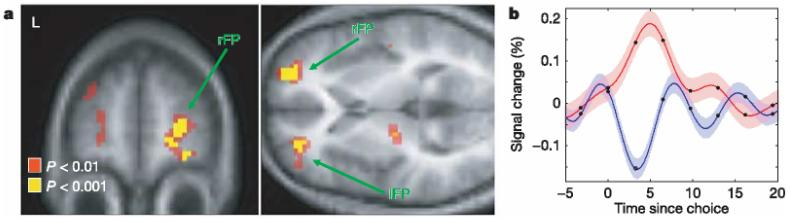
\includegraphics[width=12cm]{fig_fmri_eve.jpg}
\end{center}
\caption{In \textbf{a} shows a significance map for the difference in
  BOLD activation between exploration and exploitation trials. For the
  yellow regions the difference in BOLD activation is different from
  zero with significance $p<0.001$, for the red regions, with
  $p<0.01$. \textbf{b} shows the average time course of the BOLD
  activiation for exploration (red, mostly upper) and exploitation
  (blue, mostly lower) trials; roughly speaking, the actual data is
  marked by the black points, the lines are fitted to these
  points. [Image from \citep{DawEtAl2006}]\label{fig_fmri_eve}}
\end{figure}





\bibliographystyle{apa} \bibliography{../../source/bibliography}{}



\end{document}

